\documentclass{article}
\usepackage[utf8]{inputenc}

\title{Análisis Exploratorio de Datos \\ Trabajo Práctico 1 - Organización de Datos}
\author{Nombre de grupo}
\date{Poner fecha}

\usepackage{natbib}
\usepackage{graphicx}
\newcommand\tab[1][1cm]{\hspace*{#1}}
\usepackage{placeins}

\begin{document}
\begin{figure}
    \centering
    \makebox[\textwidth]{
\includegraphics[width=250pt]{logofiuba.jpg}}
\end{figure}

\maketitle

\FloatBarrier
\begin{center}
        \begin{tabular}{ |c|c|c| }
          \hline
          Nombre & Padrón & Mail \\
          \hline\hline
          Álvarez, Federico & 99266 & fede.alvarez1997@gmail.com \\
          \hline
          La Torre, Gabriel & 87796 & latorregab@gmail.com \\
          \hline
          Medrano, Lucas Nicolás & 99247 & lucasmedrano97@gmail.com \\
          \hline
          Piro Martino, Ariel & 99469 & ariel.piro@hotmail.com \\
          \hline
        \end{tabular}
\end{center}
\FloatBarrier

\newpage

\tableofcontents
\newpage
\section{Introduction}
	\tab En el trabajo se hace un análisis exploratorio de un set de datos provistos por la empresa Jampp. En el mismo se encuentra información de subastas, instalaciones, clicks, entre otros.\\
	\tab Primero se hará una visión general de los archivos (installs.csv, clicks.csv, auctions.csv, events.csv) para entender la distribución y la cantidad de datos, el significado de las columnas, reconocer las columnas que no aportan información (por ejemplo, las que tienen todos sus valores nulos), reconocer el tipo de datos en cada columna, seguido de un análisis mas profundo para obtener mas información de los datos. Luego se hará un análisis global, buscando información relativa a los archivos en conjunto, permitiendo obtener otro tipo de información.

\section{Análisis individual de archivos}
\subsection{Subastas}
	\subsubsection{Análisis general}
	 \tab El archivo 'auctions.csv' contiene información acerca de subastas.
	Hay dos columnas que no nos aportan información significante. 'auction\_type\_id' tiene todos sus valores 		nulos, por lo que no fue tomada en cuenta para el análisis. 'country' informa un solo valor posible, que se supone que debe ser Argentina.
	\tab La columna platforms tiene dos valores posibles (1 y 2) que se supone son Android e iOS. Va a ser importante para el análisis que hagamos más adelante.
	\tab Por último, 'source' nos da información acerca del exchange de donde surge la subasta.
	\tab Además vemos que ningún valor de este archivo, excluyendo la columna 'auction\_type\_id', es nulo, por lo que no es necesario tomar ninguna decisión respecto a eso.
	
	\subsubsection{Subastas por día de Marzo}
	\tab En el gráfico siguiente se pueden observar varias cosas:
	\begin{enumerate}
		\item La cantidad de subastas parece, en general, aumentar con el paso de los dias.
		\item El valor del último día es mas del doble del valor del primer día.
		\item El mayor aumento se da del sexto al septimo día.
		\item La cantidad de subastas se mueve entre unos valores extremos de un millón y 3 millones.
		\item para comprobar merge
	\end{enumerate}
			\begin{figure}
		    	\centering
		    	\makebox[\textwidth]{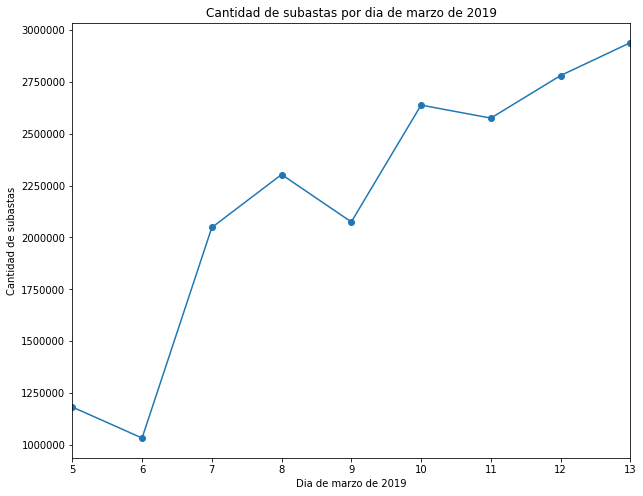
\includegraphics[width=350pt]{images/auctions/subastaspordia.png}}
		    	\caption{Subastas por día de Marzo}
			\end{figure}
	\subsubsection{Subastas por día de Marzo por sistema operativo}
	\subsubsection{Subastas por hora del día}
	\subsubsection{Subastas por día por sistema operativo}
	\subsubsection{Subastas por sistema operativo}
	\subsubsection{Subastas por source}
	

\subsection{Clicks}

\subsection{Eventos}

\subsection{Instalaciones}

\section{Análisis de archivos en conjunto}

\section{Conclusion}


\bibliographystyle{plain}
\bibliography{references}
\end{document}
